% Options for packages loaded elsewhere
\PassOptionsToPackage{unicode}{hyperref}
\PassOptionsToPackage{hyphens}{url}
%
\documentclass[
]{article}
\usepackage{amsmath,amssymb}
\usepackage{lmodern}
\usepackage{iftex}
\ifPDFTeX
  \usepackage[T1]{fontenc}
  \usepackage[utf8]{inputenc}
  \usepackage{textcomp} % provide euro and other symbols
\else % if luatex or xetex
  \usepackage{unicode-math}
  \defaultfontfeatures{Scale=MatchLowercase}
  \defaultfontfeatures[\rmfamily]{Ligatures=TeX,Scale=1}
\fi
% Use upquote if available, for straight quotes in verbatim environments
\IfFileExists{upquote.sty}{\usepackage{upquote}}{}
\IfFileExists{microtype.sty}{% use microtype if available
  \usepackage[]{microtype}
  \UseMicrotypeSet[protrusion]{basicmath} % disable protrusion for tt fonts
}{}
\makeatletter
\@ifundefined{KOMAClassName}{% if non-KOMA class
  \IfFileExists{parskip.sty}{%
    \usepackage{parskip}
  }{% else
    \setlength{\parindent}{0pt}
    \setlength{\parskip}{6pt plus 2pt minus 1pt}}
}{% if KOMA class
  \KOMAoptions{parskip=half}}
\makeatother
\usepackage{xcolor}
\usepackage[margin=1in]{geometry}
\usepackage{longtable,booktabs,array}
\usepackage{calc} % for calculating minipage widths
% Correct order of tables after \paragraph or \subparagraph
\usepackage{etoolbox}
\makeatletter
\patchcmd\longtable{\par}{\if@noskipsec\mbox{}\fi\par}{}{}
\makeatother
% Allow footnotes in longtable head/foot
\IfFileExists{footnotehyper.sty}{\usepackage{footnotehyper}}{\usepackage{footnote}}
\makesavenoteenv{longtable}
\usepackage{graphicx}
\makeatletter
\def\maxwidth{\ifdim\Gin@nat@width>\linewidth\linewidth\else\Gin@nat@width\fi}
\def\maxheight{\ifdim\Gin@nat@height>\textheight\textheight\else\Gin@nat@height\fi}
\makeatother
% Scale images if necessary, so that they will not overflow the page
% margins by default, and it is still possible to overwrite the defaults
% using explicit options in \includegraphics[width, height, ...]{}
\setkeys{Gin}{width=\maxwidth,height=\maxheight,keepaspectratio}
% Set default figure placement to htbp
\makeatletter
\def\fps@figure{htbp}
\makeatother
\setlength{\emergencystretch}{3em} % prevent overfull lines
\providecommand{\tightlist}{%
  \setlength{\itemsep}{0pt}\setlength{\parskip}{0pt}}
\setcounter{secnumdepth}{5}
\usepackage{booktabs}
\usepackage{longtable}
\usepackage{array}
\usepackage{multirow}
\usepackage{wrapfig}
\usepackage{float}
\usepackage{colortbl}
\usepackage{pdflscape}
\usepackage{tabu}
\usepackage{threeparttable}
\usepackage{threeparttablex}
\usepackage[normalem]{ulem}
\usepackage{makecell}
\usepackage{xcolor}
\ifLuaTeX
  \usepackage{selnolig}  % disable illegal ligatures
\fi
\IfFileExists{bookmark.sty}{\usepackage{bookmark}}{\usepackage{hyperref}}
\IfFileExists{xurl.sty}{\usepackage{xurl}}{} % add URL line breaks if available
\urlstyle{same} % disable monospaced font for URLs
\hypersetup{
  pdftitle={GHG\_SOIL\_DAILY\_REPORT},
  hidelinks,
  pdfcreator={LaTeX via pandoc}}

\title{GHG\_SOIL\_DAILY\_REPORT}
\author{}
\date{\vspace{-2.5em}May 05, 2025}

\begin{document}
\maketitle

{
\setcounter{tocdepth}{2}
\tableofcontents
}
\hypertarget{load-and-process-data}{%
\subsection{1. Load and Process Data}\label{load-and-process-data}}

\begin{verbatim}
## Number of rows in final_data: 30924
\end{verbatim}

\hypertarget{checking-valid-invalid}{%
\subsection{2.Checking Valid \& Invalid}\label{checking-valid-invalid}}

\begin{longtable}[t]{>{}lrr}
\caption{\label{tab:check-invalid}Summary of Invalid or Missing Rows}\\
\toprule
Row Type & Count & Percentage (\%)\\
\midrule
\textbf{\cellcolor{gray!10}{Has -9999 Only}} & \cellcolor{gray!10}{21416} & \cellcolor{gray!10}{69.3}\\
\textbf{Valid Row} & 9504 & 30.7\\
\textbf{\cellcolor{gray!10}{Has -9999 and Missing}} & \cellcolor{gray!10}{3} & \cellcolor{gray!10}{0.0}\\
\bottomrule
\end{longtable}

\begin{verbatim}
## Rows after filtering missing and -9999 values: 9504
\end{verbatim}

\hypertarget{monthyear-valid-invalid}{%
\subsection{3.MonthYear Valid \&
invalid}\label{monthyear-valid-invalid}}

\begin{longtable}[t]{>{}llrr}
\caption{\label{tab:Nan-values monthly}Monthly Summary of Invalid or Missing Rows}\\
\toprule
Month-Year & Row Type & Count & Percentage (\%)\\
\midrule
\textbf{\cellcolor{gray!10}{2024-06}} & \cellcolor{gray!10}{Has -9999 Only} & \cellcolor{gray!10}{1958} & \cellcolor{gray!10}{99.8}\\
\textbf{2024-06} & Has -9999 and Missing & 3 & 0.2\\
\textbf{\cellcolor{gray!10}{2024-07}} & \cellcolor{gray!10}{Has -9999 Only} & \cellcolor{gray!10}{6557} & \cellcolor{gray!10}{100.0}\\
\textbf{2024-08} & Has -9999 Only & 6122 & 100.0\\
\textbf{\cellcolor{gray!10}{2024-09}} & \cellcolor{gray!10}{Has -9999 Only} & \cellcolor{gray!10}{4396} & \cellcolor{gray!10}{100.0}\\
\addlinespace
\textbf{2024-10} & Has -9999 Only & 192 & 100.0\\
\textbf{\cellcolor{gray!10}{2024-11}} & \cellcolor{gray!10}{Has -9999 Only} & \cellcolor{gray!10}{721} & \cellcolor{gray!10}{12.5}\\
\textbf{2024-11} & Valid Row & 5031 & 87.5\\
\textbf{\cellcolor{gray!10}{2024-12}} & \cellcolor{gray!10}{Has -9999 Only} & \cellcolor{gray!10}{1366} & \cellcolor{gray!10}{24.1}\\
\textbf{2024-12} & Valid Row & 4300 & 75.9\\
\addlinespace
\textbf{\cellcolor{gray!10}{2025-04}} & \cellcolor{gray!10}{Has -9999 Only} & \cellcolor{gray!10}{104} & \cellcolor{gray!10}{37.5}\\
\textbf{2025-04} & Valid Row & 173 & 62.5\\
\bottomrule
\end{longtable}

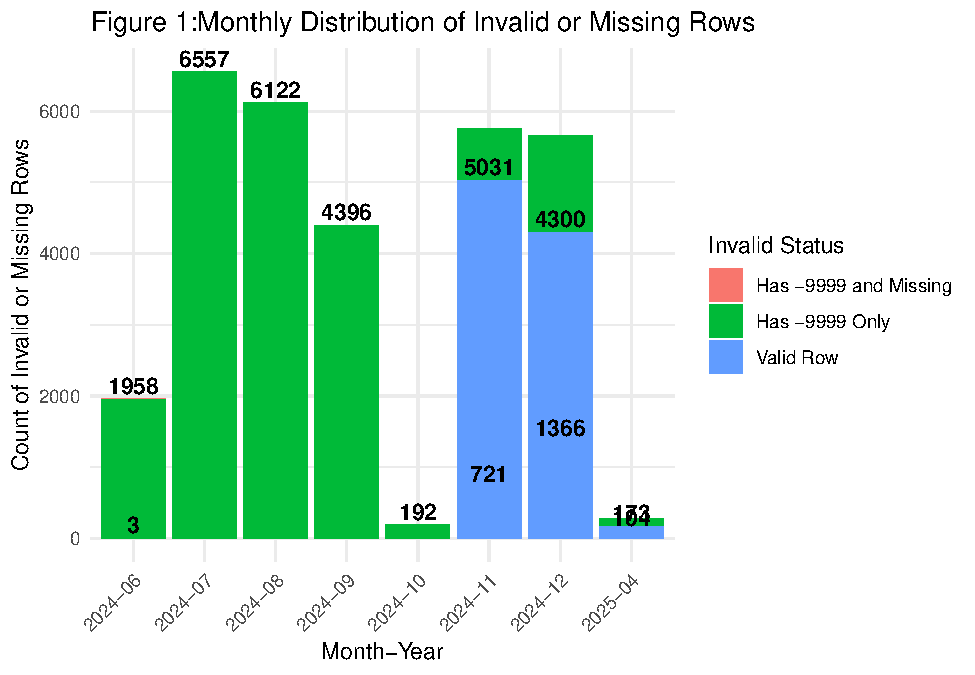
\includegraphics{/lustre/darse/users/3735/ghgsoilproject/output/GHG_SOIL_REPORT_2025-05-05_files/figure-latex/Nan-values monthly-1.pdf}

\hypertarget{sensor-failures}{%
\subsection{4. Sensor Failures}\label{sensor-failures}}

\begin{longtable}[t]{>{}lrrrr}
\caption{\label{tab:sensor-failures}Monthly Summary of Rows with -9999 in Specific Columns}\\
\toprule
MonthYear & TotalRows & RowsWith\_One\_Column & RowsWith\_Multiple\_Columns & RowsWith\_All\_Columns\\
\midrule
\textbf{\cellcolor{gray!10}{2024-06}} & \cellcolor{gray!10}{1961} & \cellcolor{gray!10}{NA} & \cellcolor{gray!10}{NA} & \cellcolor{gray!10}{0}\\
\textbf{2024-07} & 6557 & 4874 & 1683 & 0\\
\textbf{\cellcolor{gray!10}{2024-08}} & \cellcolor{gray!10}{6122} & \cellcolor{gray!10}{4970} & \cellcolor{gray!10}{1152} & \cellcolor{gray!10}{0}\\
\textbf{2024-09} & 4396 & 3763 & 633 & 0\\
\textbf{\cellcolor{gray!10}{2024-10}} & \cellcolor{gray!10}{192} & \cellcolor{gray!10}{168} & \cellcolor{gray!10}{24} & \cellcolor{gray!10}{0}\\
\addlinespace
\textbf{2024-11} & 5752 & 0 & 721 & 0\\
\textbf{\cellcolor{gray!10}{2024-12}} & \cellcolor{gray!10}{5666} & \cellcolor{gray!10}{0} & \cellcolor{gray!10}{1366} & \cellcolor{gray!10}{0}\\
\textbf{2025-04} & 277 & 0 & 104 & 0\\
\bottomrule
\end{longtable}

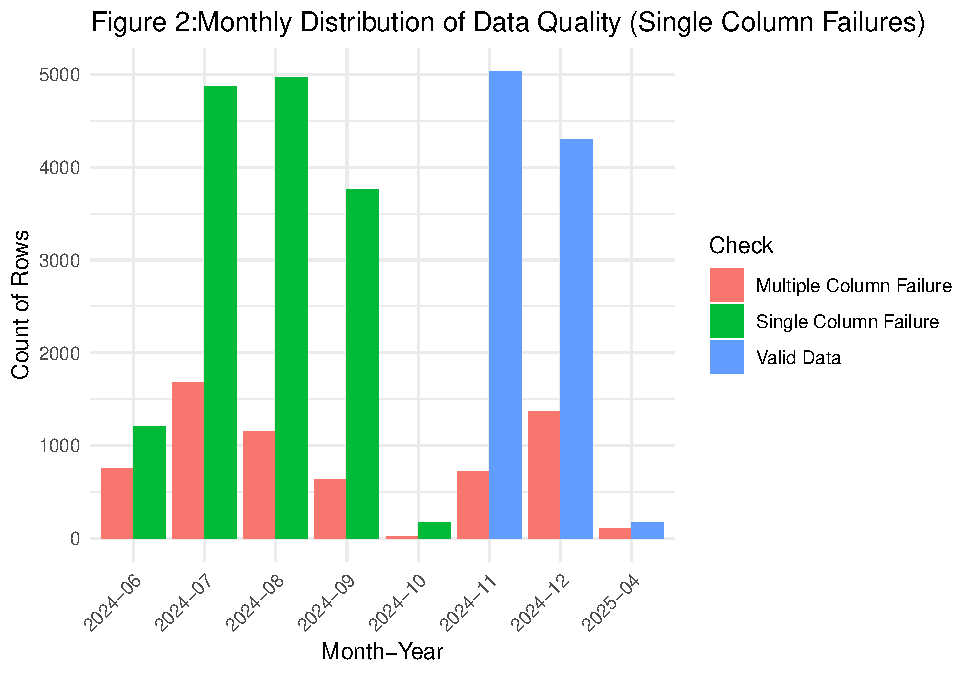
\includegraphics{/lustre/darse/users/3735/ghgsoilproject/output/GHG_SOIL_REPORT_2025-05-05_files/figure-latex/sensor-failures-1.pdf}

\hypertarget{corelation-matrix}{%
\subsection{5. Corelation Matrix}\label{corelation-matrix}}

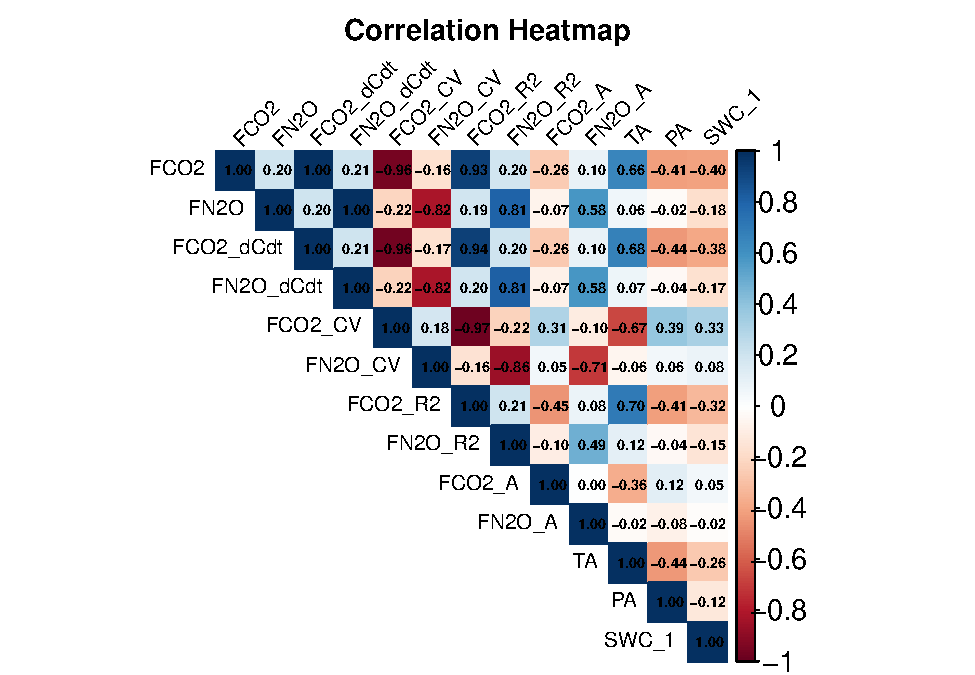
\includegraphics{/lustre/darse/users/3735/ghgsoilproject/output/GHG_SOIL_REPORT_2025-05-05_files/figure-latex/corelation matrix-1.pdf}
\#\# 5. Time Gap Categorization \& Flagging

\begin{verbatim}
##               DateTime TimeDiff_min  GapCategory   TimeGapFlag
## 1  2024-07-12 15:00:41   4720.75000   1 - 5 days Very Long Gap
## 2  2024-07-18 17:00:41   1860.00000   1 - 5 days Very Long Gap
## 3  2024-08-02 11:44:53     92.53333  1 - 6 hours      Long Gap
## 4  2024-08-02 14:00:41     77.36667  1 - 6 hours      Long Gap
## 5  2024-08-07 12:00:41     94.10000  1 - 6 hours      Long Gap
## 6  2024-08-30 17:00:41    514.10000 6 - 12 hours      Long Gap
## 7  2024-09-09 15:00:41    348.90000  1 - 6 hours      Long Gap
## 8  2024-09-09 17:00:41    101.50000  1 - 6 hours      Long Gap
## 9  2024-09-25 18:00:41    585.26667 6 - 12 hours      Long Gap
## 10 2024-09-29 16:07:26   4315.71667   1 - 5 days Very Long Gap
## 11 2024-09-30 11:00:41     94.10000  1 - 6 hours      Long Gap
## 12 2024-11-24 13:00:41    154.20000  1 - 6 hours      Long Gap
## 13 2024-12-12 15:00:42    394.21667 6 - 12 hours      Long Gap
## 14 2024-12-17 16:00:42    120.00000  1 - 6 hours      Long Gap
## 15 2024-12-19 14:00:41    274.90000  1 - 6 hours      Long Gap
## 16 2025-04-14 15:00:51    136.70000  1 - 6 hours      Long Gap
\end{verbatim}

\hypertarget{summary-visualization}{%
\subsection{6. Summary \& Visualization}\label{summary-visualization}}

\begin{verbatim}
## [1] "Skewness of TimeDiff_min: 45.61"
\end{verbatim}

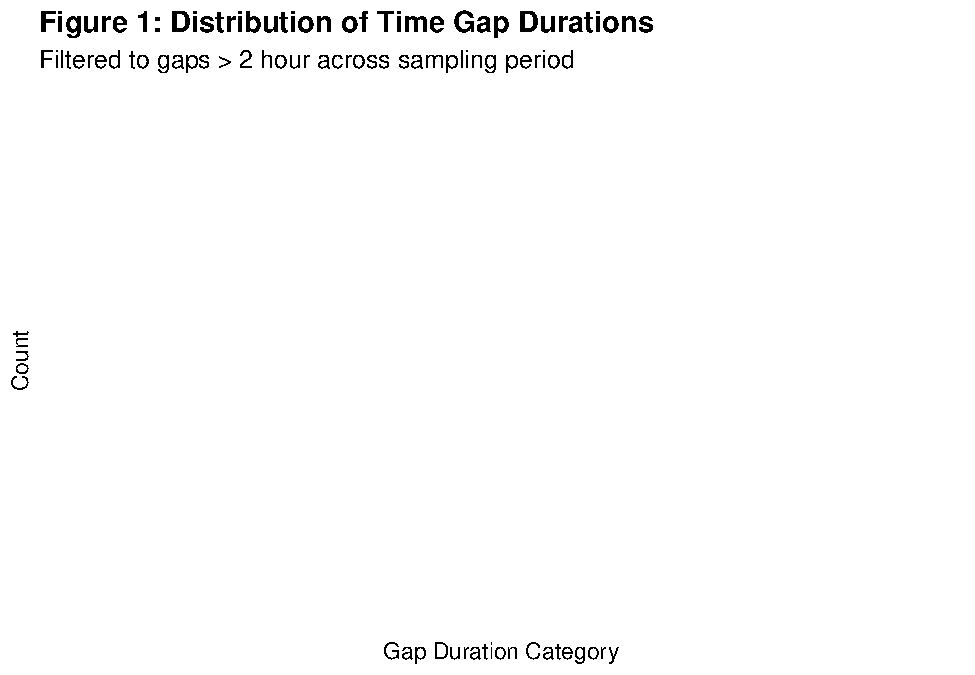
\includegraphics{/lustre/darse/users/3735/ghgsoilproject/output/GHG_SOIL_REPORT_2025-05-05_files/figure-latex/summary-1.pdf}

\hypertarget{monthly-trends-power-outages}{%
\subsection{7. Monthly Trends \& Power
Outages}\label{monthly-trends-power-outages}}

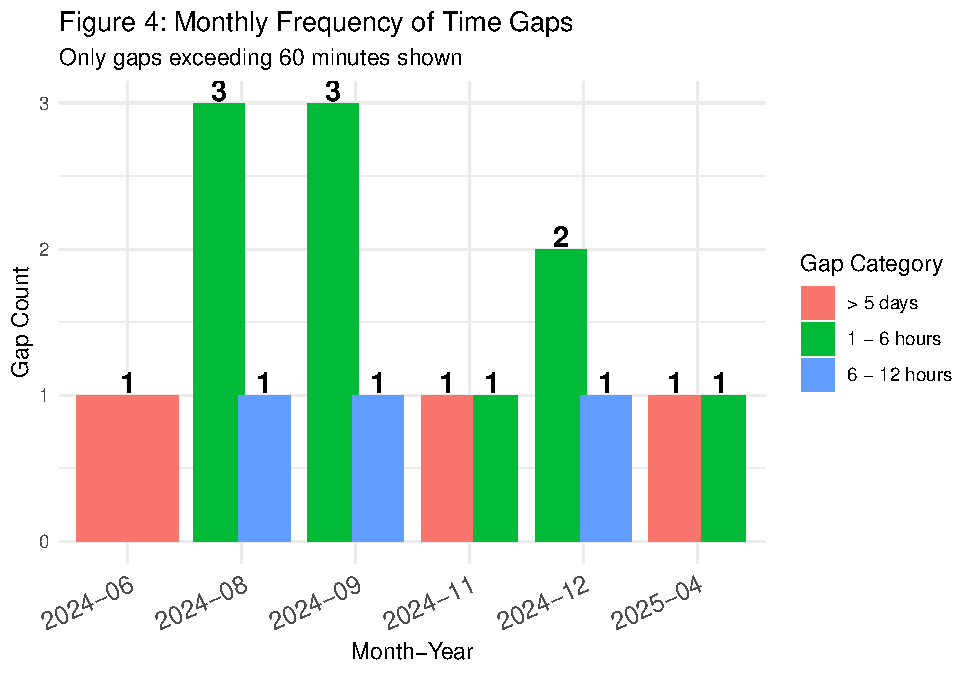
\includegraphics{/lustre/darse/users/3735/ghgsoilproject/output/GHG_SOIL_REPORT_2025-05-05_files/figure-latex/monthly-trends-1.pdf}

\hypertarget{r2-analysis}{%
\subsection{8. R2 Analysis}\label{r2-analysis}}

\begin{longtable}[t]{rrrrr}
\caption{\label{tab:r2 analysis}Summary of R² Values for CO2 Flux (FCO2)}\\
\toprule
Total Records & R² >= 0.75 & R² < 0.75 & Percentage ≥ 0.75 & Percentage < 0.75\\
\midrule
\cellcolor{gray!10}{9504} & \cellcolor{gray!10}{7669} & \cellcolor{gray!10}{1835} & \cellcolor{gray!10}{80.7} & \cellcolor{gray!10}{19.3}\\
\bottomrule
\end{longtable}

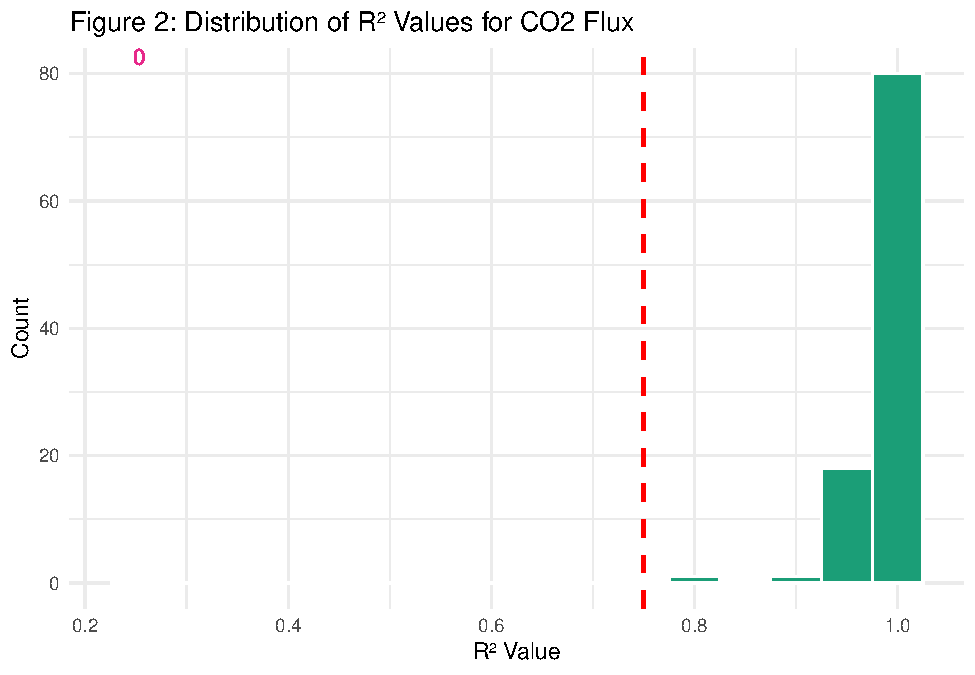
\includegraphics{/lustre/darse/users/3735/ghgsoilproject/output/GHG_SOIL_REPORT_2025-05-05_files/figure-latex/r2 analysis-1.pdf}
\#\# 9. CV Analysis

\begin{longtable}[]{@{}lrr@{}}
\caption{Summary of CO2 Flux CV Flags}\tabularnewline
\toprule()
CO2 Flux CV Flag & Count & Percentage \\
\midrule()
\endfirsthead
\toprule()
CO2 Flux CV Flag & Count & Percentage \\
\midrule()
\endhead
Acceptable & 2165 & 22.8 \\
Issue & 4430 & 46.6 \\
Plausible & 2909 & 30.6 \\
\bottomrule()
\end{longtable}

\begin{longtable}[]{@{}lrr@{}}
\caption{Summary of N2O Flux CV Flags}\tabularnewline
\toprule()
N2O Flux CV Flag & Count & Percentage \\
\midrule()
\endfirsthead
\toprule()
N2O Flux CV Flag & Count & Percentage \\
\midrule()
\endhead
Acceptable & 163 & 1.7 \\
Issue & 9296 & 97.8 \\
Plausible & 45 & 0.5 \\
\bottomrule()
\end{longtable}

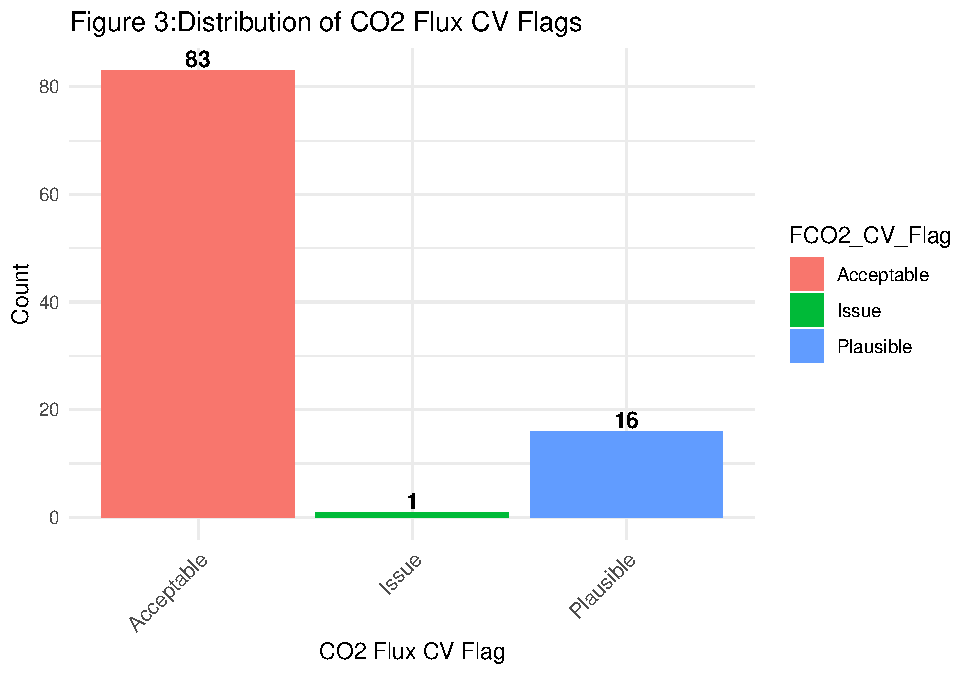
\includegraphics{/lustre/darse/users/3735/ghgsoilproject/output/GHG_SOIL_REPORT_2025-05-05_files/figure-latex/cv analysis-1.pdf}
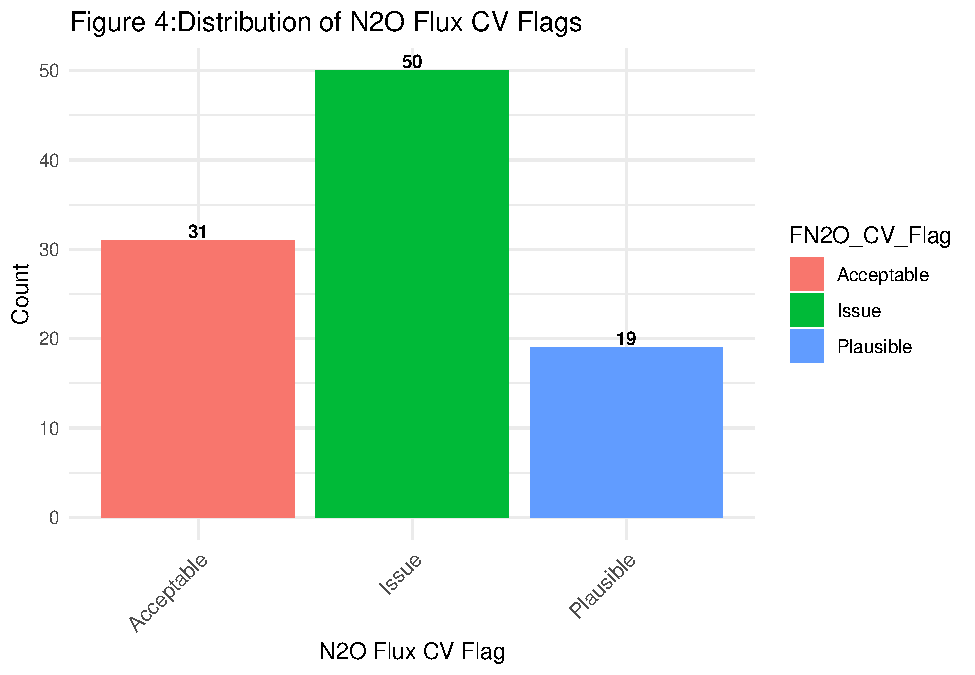
\includegraphics{/lustre/darse/users/3735/ghgsoilproject/output/GHG_SOIL_REPORT_2025-05-05_files/figure-latex/cv analysis-2.pdf}

\hypertarget{flux-control}{%
\subsection{10. Flux Control}\label{flux-control}}

\begin{longtable}[]{@{}lrr@{}}
\caption{Summary of CO2 Flux Flags}\tabularnewline
\toprule()
CO Flux Flag & Count & Percentage \\
\midrule()
\endfirsthead
\toprule()
CO Flux Flag & Count & Percentage \\
\midrule()
\endhead
Very Low (\textless100) & 7669 & 100 \\
\bottomrule()
\end{longtable}

\begin{longtable}[]{@{}lrr@{}}
\caption{Summary of N2O Flux Flags}\tabularnewline
\toprule()
NO Flux Flag & Count & Percentage \\
\midrule()
\endfirsthead
\toprule()
NO Flux Flag & Count & Percentage \\
\midrule()
\endhead
Below Detection (\textless0.01) & 760 & 9.9 \\
Extremely High (\textgreater5) & 4 & 0.1 \\
Negative & 693 & 9.0 \\
Plausible & 6212 & 81.0 \\
\bottomrule()
\end{longtable}

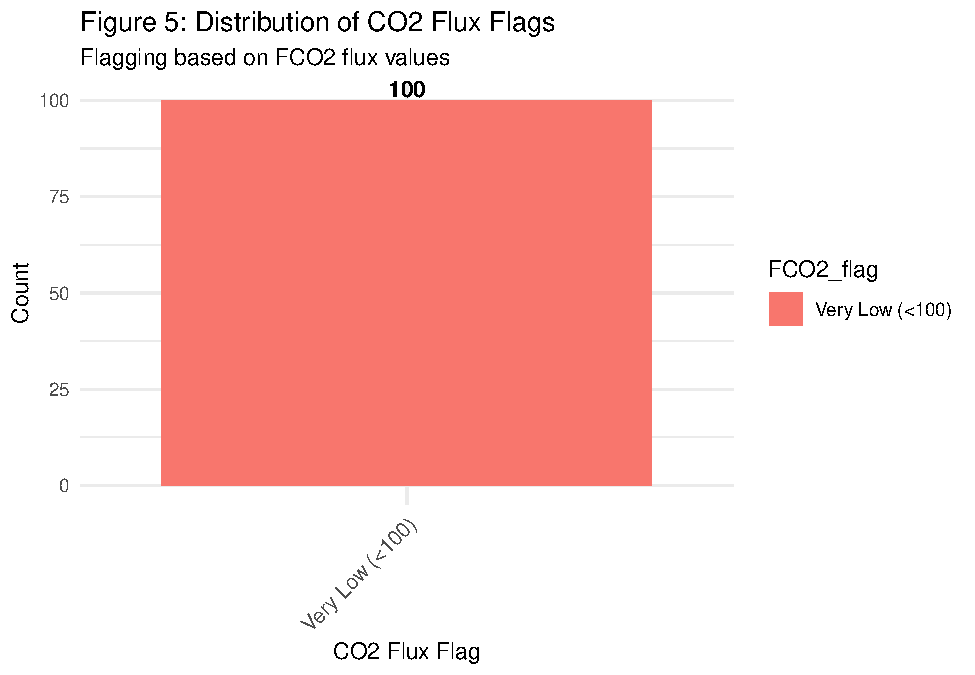
\includegraphics{/lustre/darse/users/3735/ghgsoilproject/output/GHG_SOIL_REPORT_2025-05-05_files/figure-latex/flux-quality-control-1.pdf}
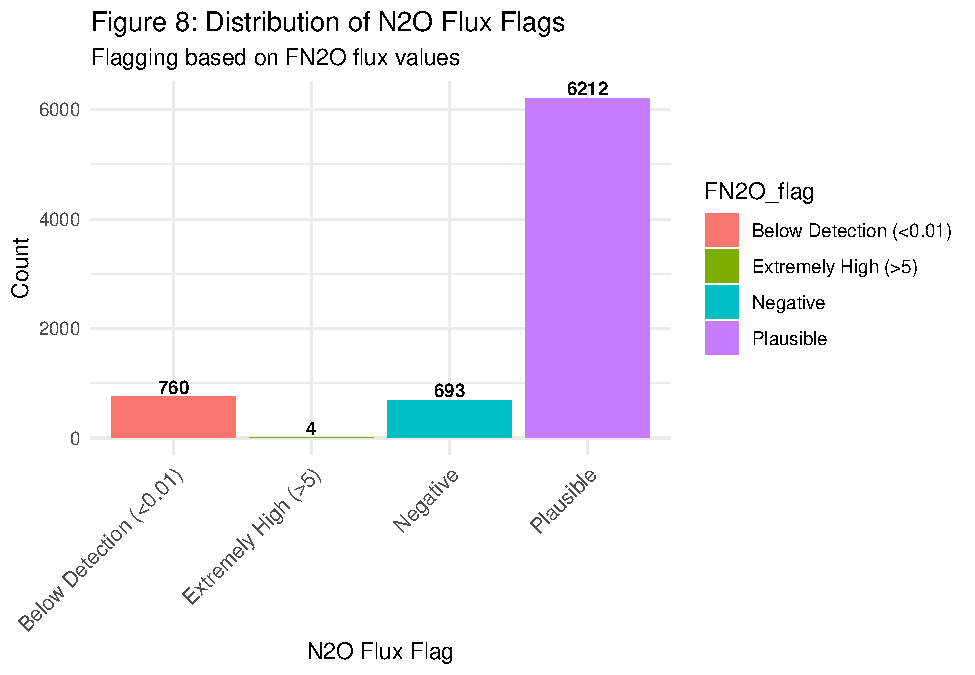
\includegraphics{/lustre/darse/users/3735/ghgsoilproject/output/GHG_SOIL_REPORT_2025-05-05_files/figure-latex/flux-quality-control-2.pdf}

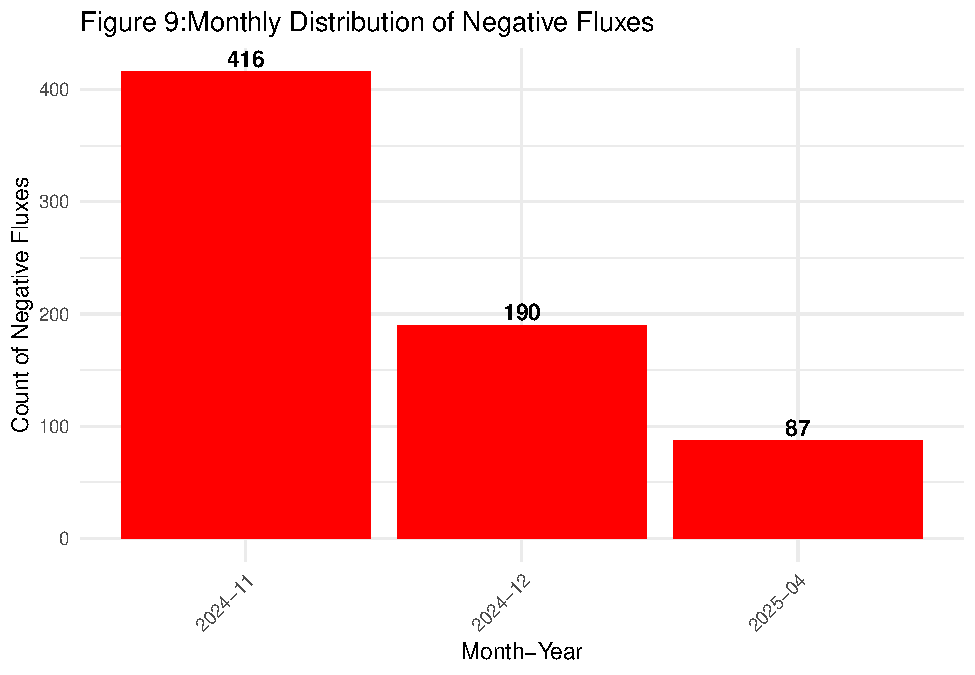
\includegraphics{/lustre/darse/users/3735/ghgsoilproject/output/GHG_SOIL_REPORT_2025-05-05_files/figure-latex/flux anlysis monthly-1.pdf}
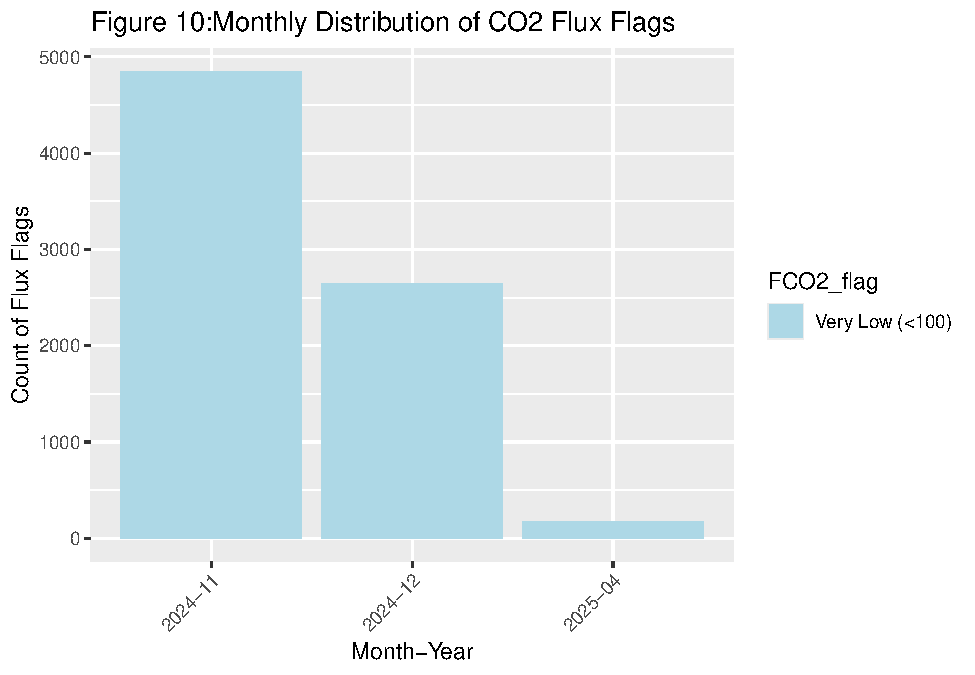
\includegraphics{/lustre/darse/users/3735/ghgsoilproject/output/GHG_SOIL_REPORT_2025-05-05_files/figure-latex/flux anlysis monthly-2.pdf}
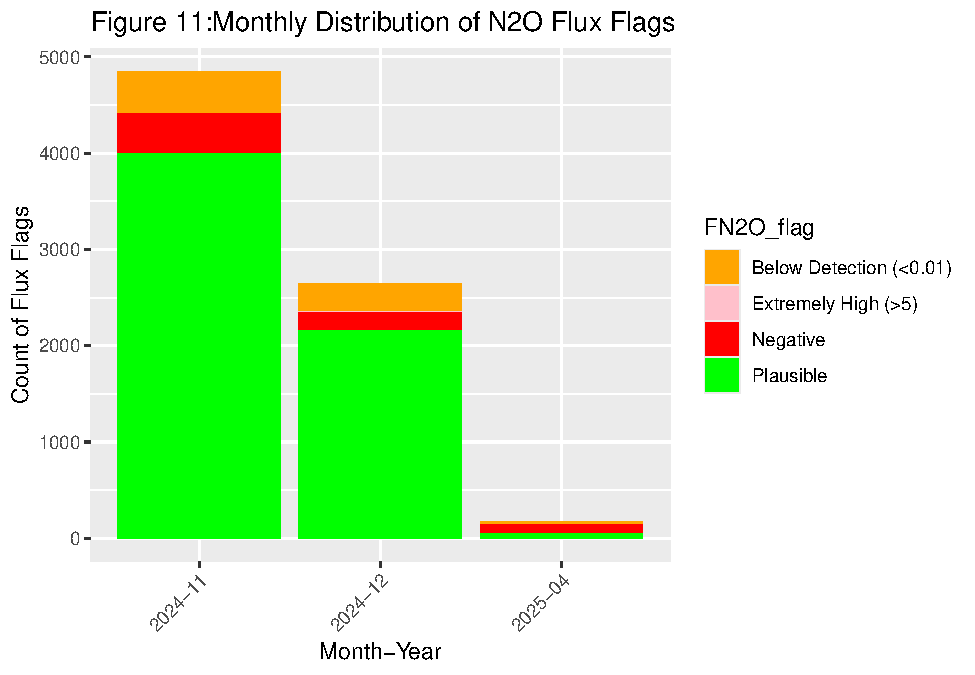
\includegraphics{/lustre/darse/users/3735/ghgsoilproject/output/GHG_SOIL_REPORT_2025-05-05_files/figure-latex/flux anlysis monthly-3.pdf}

\end{document}
